\chapter{Resultados}\label{chp:res}

O conjunto de dados, originais e derivados (aqueles criados a partir de dados originais), estão apresentados na tabela \ref{tab:all_data_table}.

\begin{table}[]
\centering
\resizebox{\textwidth}{!}{\begin{tabular}{|l|c|c|c|c|}
\hline
Plataforma & \multicolumn{4}{c|}{Dado} \\ \hline
 & \multicolumn{4}{l|}{} \\ \hline
Sensor & Tempo & Mensagem & Tamanho do arquivo \\ \hline
Giroscopio & Taxa de giro em X & Taxa de giro em Y & Taxa de giro em Z &  \\ \hline
Acelerometro & Aceleração em X & Aceleração em Y & Aceleração em Z &  \\ \hline
Pitot & Raw Pitot - Pitot 0 & Pressao Dinamica Ref.- Pitot 0 (virtual) & Velocidade Ref. - Pitot 0 (virtual) &  \\ \hline
Pitot & Raw Pitot - Pitot 1 & Pressao Dinamica Ref.- Pitot 1 (virtual) & Velocidade Ref. - Pitot 1 (virtual) &  \\ \hline
Pitot & Raw Pitot - Pitot 2 & Pressao Dinamica Ref.- Pitot 2 (virtual) & Velocidade Ref. - Pitot 2 (virtual) &  \\ \hline
Pitots & AoA Differential Pressure - Sonda AoA (virtual) 0 & AoA Dynamic Pressure - Sonda AoA 0 (virtual) & AoA - Sonda AoA 0 (virtual) &  \\ \hline
Célula de carga & Raw Cell Data - Celula Horizontal & Forca - Celula Horizontal (virtual) &  &  \\ \hline
Célula de carga & Raw Cell Data - Celula Frontal Direita & Forca - Celula Frontal Direita (virtual) &  &  \\ \hline
Célula de carga & Raw Cell Data - Celula Frontal Esquerda & Forca - Celula Frontal Esquerda (virtual) &  &  \\ \hline
Célula de carga & Raw Cell Data - Celula Traseira Direita & Forca - Celula Traseira Direita (virtual) &  &  \\ \hline
Célula de carga & Raw Cell Data - Celula Traseira Esquerda & Forca - Celula Traseira Esquerda (virtual) &  &  \\ \hline
Células de carga e Pitots & Lift (virtual) & Drag (virtual) & Moment (virtual) & Distance Cp (virtual) \\ \hline
\end{tabular}}
\caption{Dados disponíveis no arquivo gerado pela plataforma de aquisição}
\label{tab:all_data_table}
\end{table}

Na imagem \ref{fig:raw_accel_plots} pode ser visto um exemplo dos dados adquiridos durante uma bateria de testes. A gravação dos dados na plataforma ocorre a uma taxa fixa de 100 Hz, diferente da taxa original de aquisição de cada sensor. 

Isso é feito de modo que todos apresentem uma mesma frequência de ocorrência na plataforma e portanto tenham sempre correspondência nos dados dos outros sensores, facilitando posterior processamento. Neste nivelamento alguns dados, por possuírem frequência de aquisição mais baixa que a de gravação da plataforma, acabam se repetindo até que novos valores estejam disponíveis.

\begin{figure}[!ht]
    \centering
    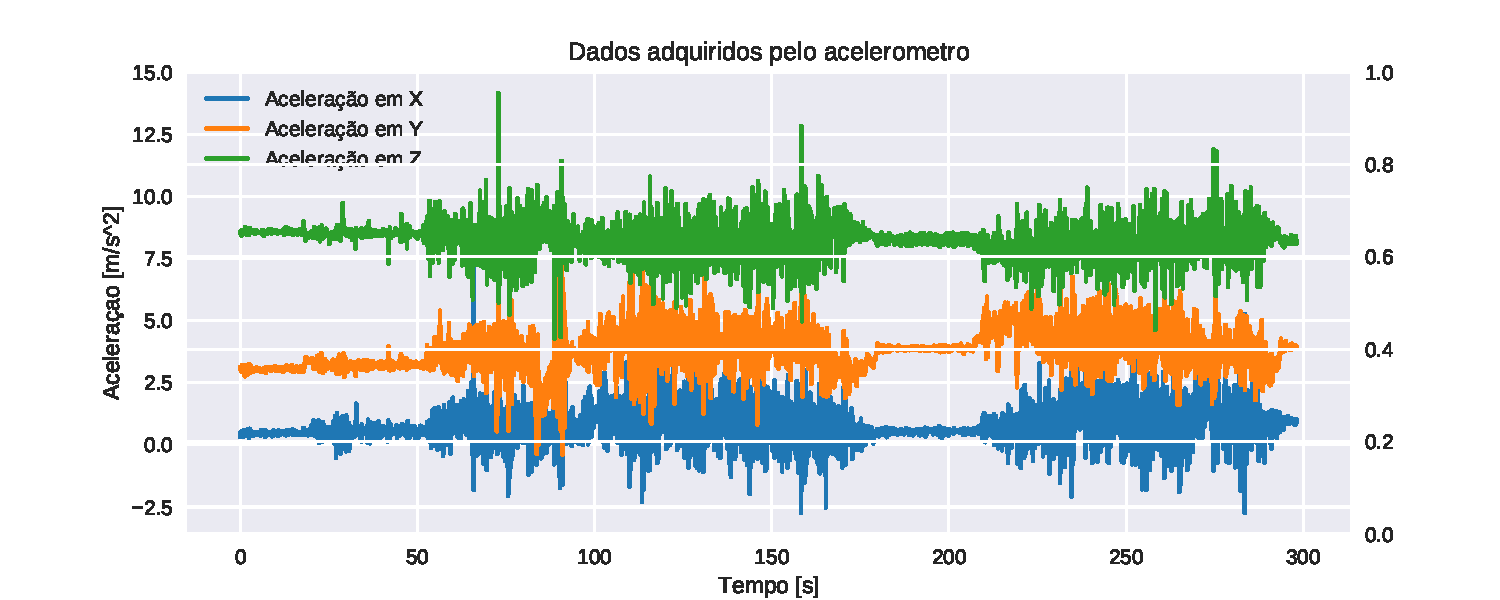
\includegraphics[width=.8\linewidth]{plots/accel_plots.pdf}
    \caption{Exemplo de dados do acelerômetro. Fonte: O autor.}
    \label{fig:raw_accel_plots}
\end{figure}

\begin{figure}[!ht]
    \centering
    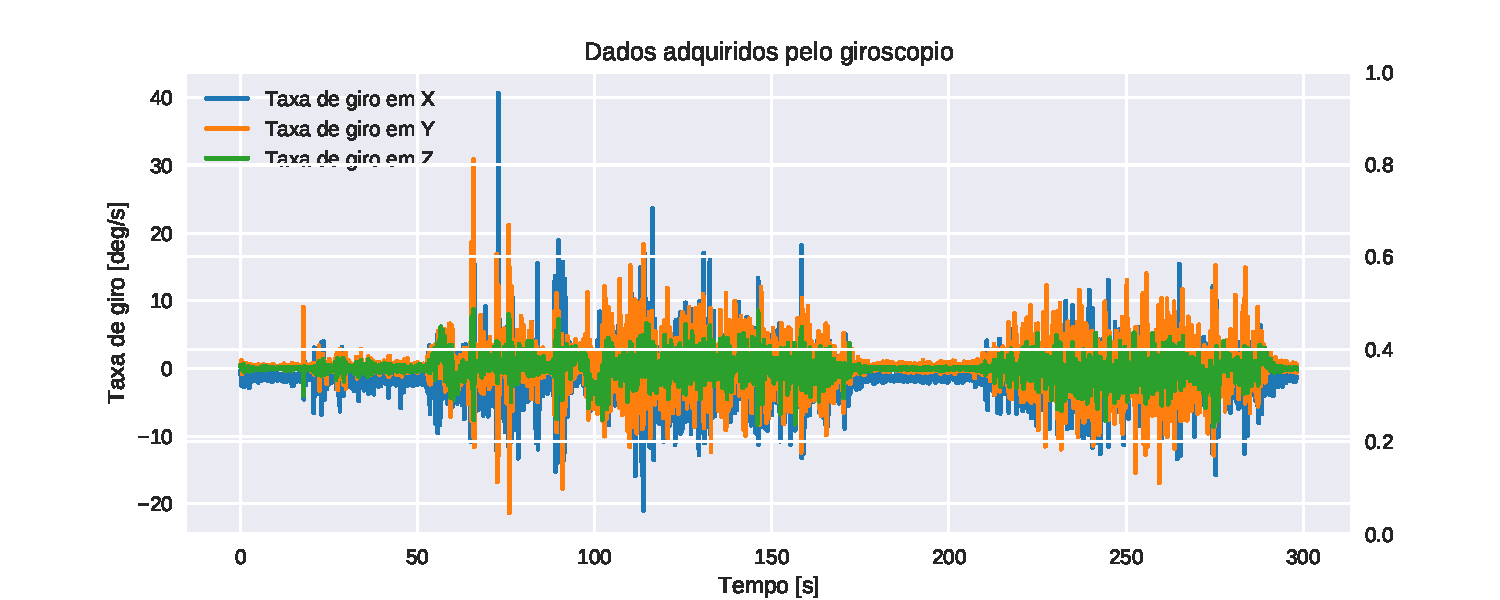
\includegraphics[width=.8\linewidth]{plots/gyro_plots.pdf}
    \caption{Exemplo de dados do giroscópio. Fonte: O autor.}
    \label{fig:raw_gyro_plots}
\end{figure}

\begin{figure}[!ht]
    \centering
    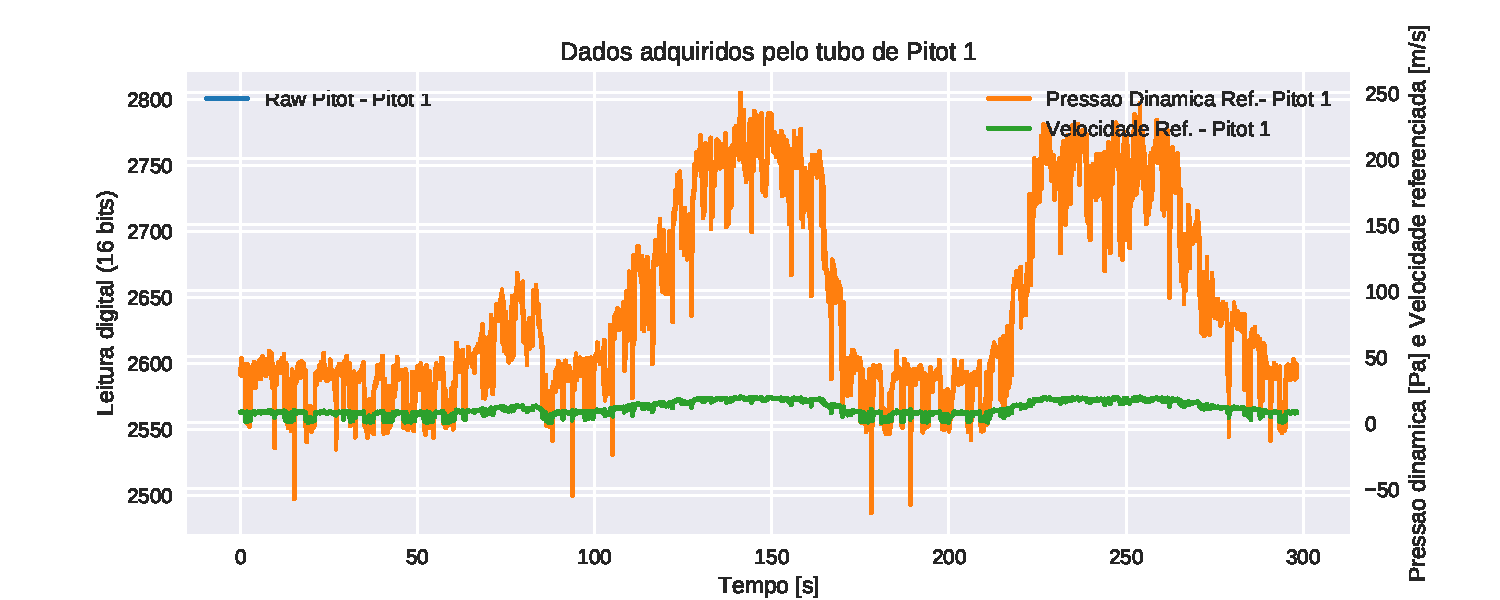
\includegraphics[width=.8\linewidth]{plots/pitot_plots.pdf}
    \caption{Exemplo de dados do Pitot. Fonte: O autor.}
    \label{fig:raw_pitot_plots}
\end{figure}

\begin{figure}[!ht]
    \centering
    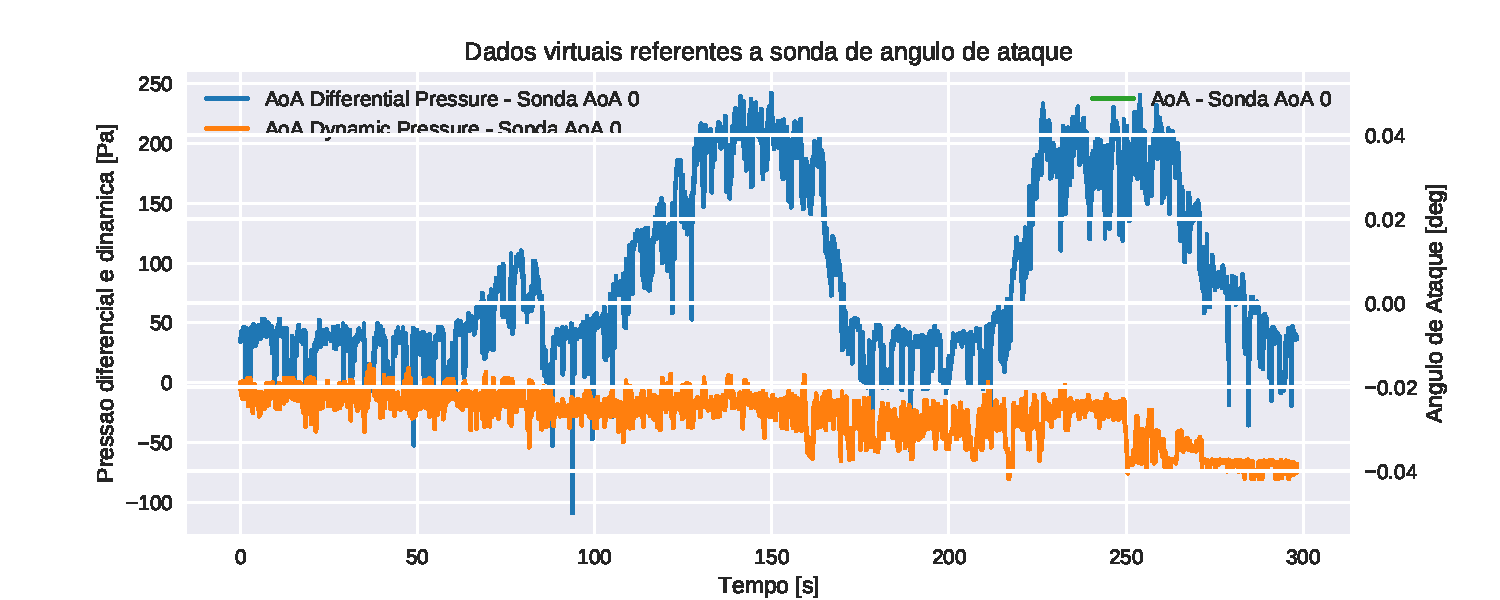
\includegraphics[width=.8\linewidth]{plots/aoa_plots.pdf}
    \caption{Exemplo de dados da sonda de angulo de ataque. Fonte: O autor.}
    \label{fig:raw_aoa_plots}
\end{figure}

\begin{figure}[!ht]
    \centering
    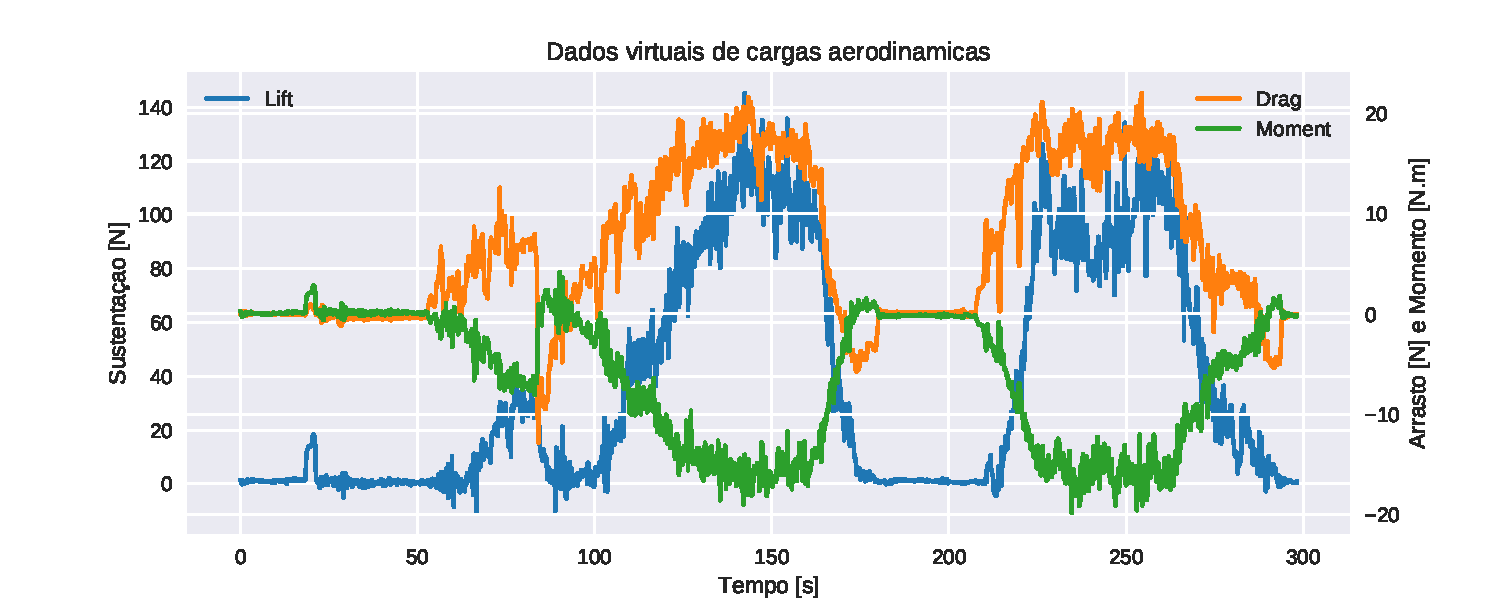
\includegraphics[width=.8\linewidth]{plots/loads_plots.pdf}
    \caption{Exemplo de dados de cargas aerodinâmicas. Fonte: O autor.}
    \label{fig:raw_load_plots}
\end{figure}

\section{Limpeza, filtragem e redução dos dados}

\subsection{Limpeza de dados}

Dado que o teste foi executado procurando-se atingir uma velocidade constante, o resultado final será dado para apenas um valor de Reynolds, sendo assim, dados adquiridos que sejam válidos mas não estejam próximos ao Reynolds do teste não devem ser utilizados, dado que devem apresentar comportamento aerodinâmico diferente daquele correspondente ao Reynolds desejado \citep{anderson1984fundamentals}. Sendo assim, a primeira limpeza a ser realizada é quanto à faixa de interesse de Reynolds. Desta forma os dados a serem utilizados para medição serão aqueles correspondentes aos instantes onde foi alcançada a velocidade estipulada para o teste, com desvio máximo de 10\%.

Para mostrar o resultado desta filtragem usaremos os dados de Sustentação. Os dados originais se encontram na figura \ref{fig:orig_lift_plot} enquanto os dados após filtragem por faixa de Reynolds se encontram na figura \ref{fig:lift_reynolds_filter} :

\begin{figure}[!ht]
    \centering
    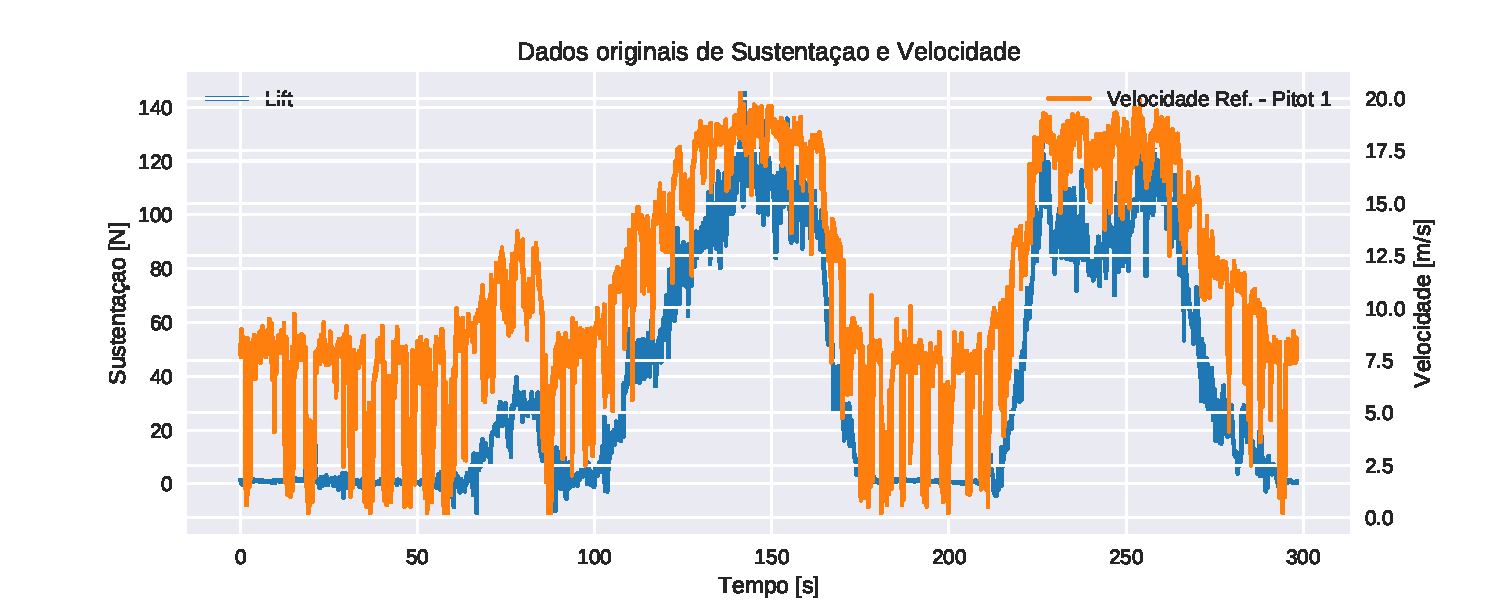
\includegraphics[width=.8\linewidth]{plots/orig_lift_plot.pdf}
    \caption{Dados de sustentação e velocidade originais. Fonte: O autor.}
    \label{fig:orig_lift_plot}
\end{figure}


\begin{figure}[!ht]
    \centering
    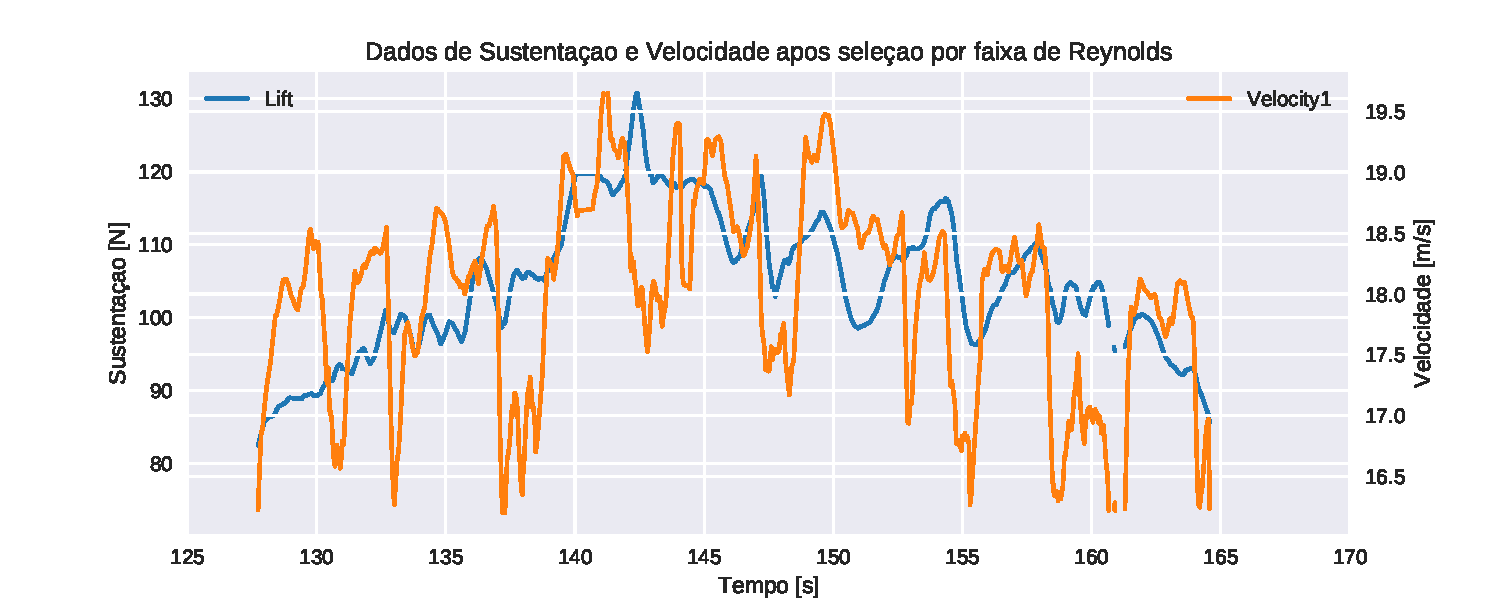
\includegraphics[width=.8\linewidth]{plots/reynolds_lift_plot.pdf}
    \caption{Dados de sustentação e velocidade após filtragem pela faixa de Reynolds do teste (1o patamar). Fonte: O autor.}
    \label{fig:lift_reynolds_filter}
\end{figure}

% A premissa principal para o uso dos dados do teste é de que os valores medidos estejam dentro do intervalo de uso dos sensores e de que as acelerações sobre o sistema sejam baixas. O intervalo de uso dos sensores se encontra na tabela X.

% \begin{table}[!ht]
%     \centering
%     
\includegraphics[width=.8\linewidth]{figuras/outras/placeholder.png}
%     \caption{TABELA COM ZONA DE USO DE CADA SENSOR. Fonte: O autor.}
%     \label{fig:placeholder}
% \end{table}

% Após a seleção por faixa de Reynolds, dados fora da faixa de medição dos sensores e dados com aceleração em X, Y ou Z maior que 0.5g foram também descartados.

\subsection{Filtragem}

Após a limpeza dos dados, onde foram removidos aqueles que estavam fora da zona de interesse, buscou-se avaliar a filtragem do sinal, visando aumentar a relação sinal-ruido.

Primeiramente foram realizadas Transformadas Rápidas de Fourier nos dados das células e das sondas de angulo de ataque (incluindo velocidade). Através da transformação para o domínio da frequência foi possível encontrar as frequências de corte ideais para aplicação de filtros passa-baixa em cada um dos dados.

% \begin{figure}[!ht]
%     \centering
%     \includegrapha apoliics[width=.8\linewidth]{figuras/outras/placeholder.png}
%     \caption{ANALISES FFT. Fonte: O autor.}
%     \label{fig:fft_analysis}
% \end{figure}

% A partir do resultado das analises foram dimensionados filtros do tipo passa-baixa para a remoção dos ruídos de alta frequência em cada um dos dados.

% As frequências de corte para cada dado se encontram na tabela X. 

% \begin{table}[!ht]
%     \centering
%     
\includegraphics[width=.6\linewidth]{figuras/outras/placeholder.png}
%     \caption{TABELA COM FREQUENCIA DE CORTE DE CADA DADO. Fonte: O autor.}
%     \label{tab:cut_frequency_values}
% \end{table}

A titulo de exemplo, o resultado após filtragem para os dados de sustentação e velocidade se encontram na figura \ref{fig:filtered_lift_plot}.

\begin{figure}[!ht]
    \centering
    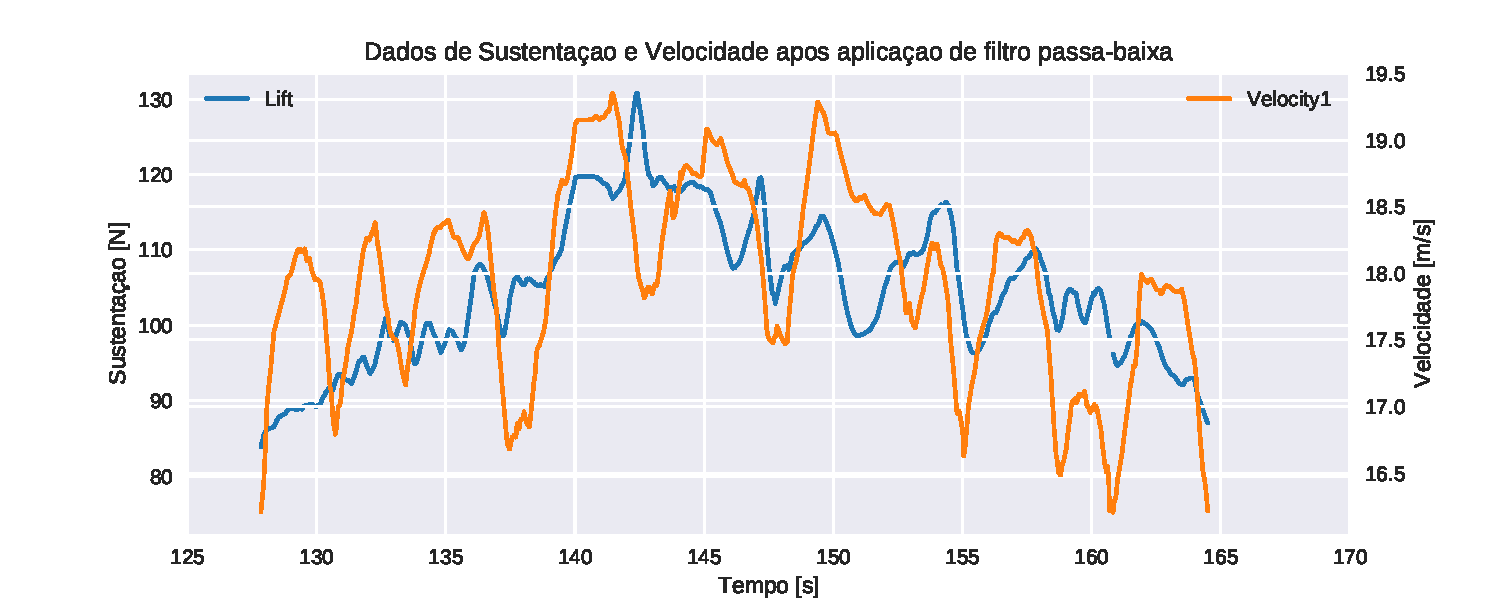
\includegraphics[width=.8\linewidth]{plots/filtered_lift_plot.pdf}
    \caption{Dados de sustentação e velocidade após filtragem das altas frequências. Fonte: O autor.}
    \label{fig:filtered_lift_plot}
\end{figure}

\subsection{Redução}

Em posse dos dados filtrados passa-se à etapa de redução. Não é do interesse do projetista a principio saber qual sustentação, arrasto ou momento foram alcançados durante os testes, pois esses são dados absolutos que dependem do tamanho do componente e da velocidade no instante medido. Para facilidade de analise e mais justa comparação entre diferentes componentes é de interesse a redução destes dados na forma dos coeficientes aerodinâmicos \citep{anderson1984fundamentals}.

\begin{equation}
    C_L =  \frac{L}{ \frac{1}{2} \rho V^{2} S}
    \label{eq:cl}
\end{equation}

\begin{equation} 
    C_D =  \frac{D}{ \frac{1}{2} \rho V^{2} S}
    \label{eq:cd}
\end{equation}

\begin{equation}
    C_M =  \frac{M}{ \frac{1}{2} \rho V^{2} S C_{M.A.}} 
    \label{eq:cm}
\end{equation}

As equações \ref{eq:cl}, \ref{eq:cd} e \ref{eq:cm} foram aplicadas a todas as amostras de dados gerando três novas colunas, $C_L$, $C_D$ e $C_M$, que podem ser visualizadas na figura \ref{fig:coefficients_plot}. Os dados das baterias de testes foram então condensados num mesmo conjunto de dados,para o qual então foram calculados o valor médio e o desvio padrão de cada coeficiente, para cada angulo de incidência.

\begin{figure}[!ht]
    \centering
    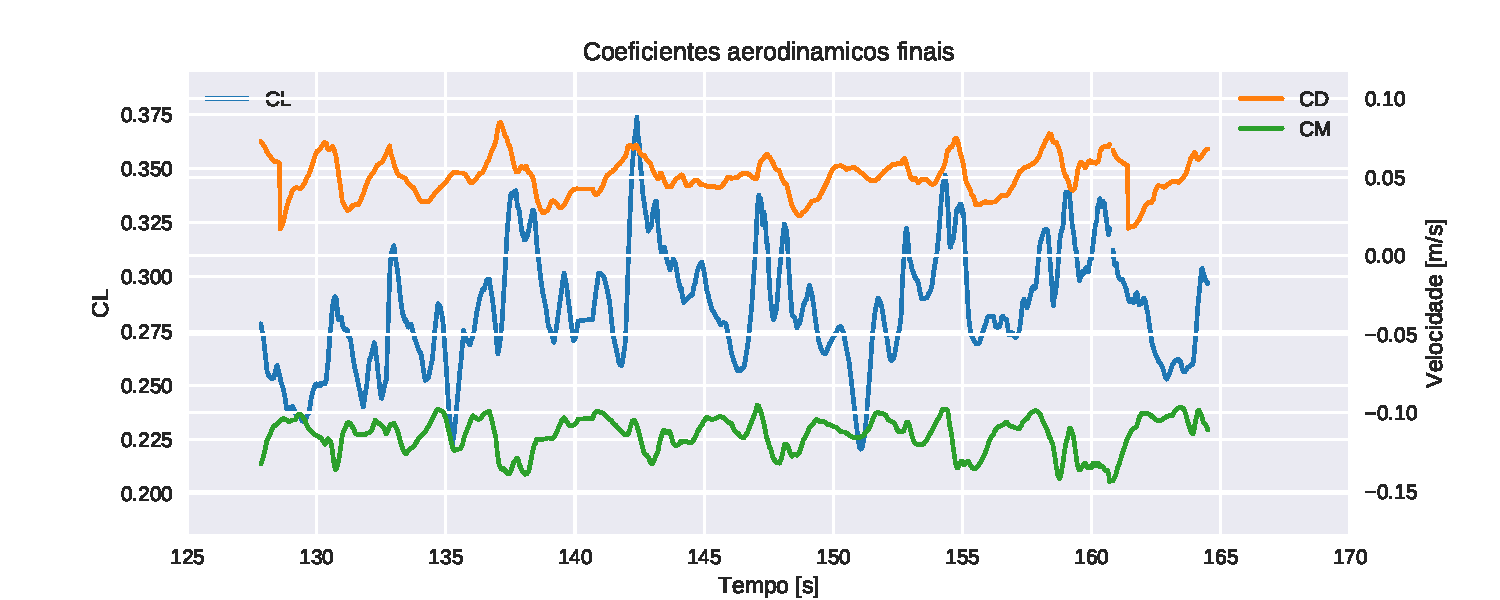
\includegraphics[width=.8\linewidth]{plots/coefficients_plot.pdf}
    \caption{Variação dos coeficientes aerodinâmicos ao longo do tempo para o patamar avaliado. Fonte: O autor.}
    \label{fig:coefficients_plot}
\end{figure}

Os valores finais de media para os coeficientes de cada angulo de incidência estão explicitados nos gráficos da figura \ref{fig:coefficients_alpha_plot}.

\begin{figure}[!ht]
    \centering
    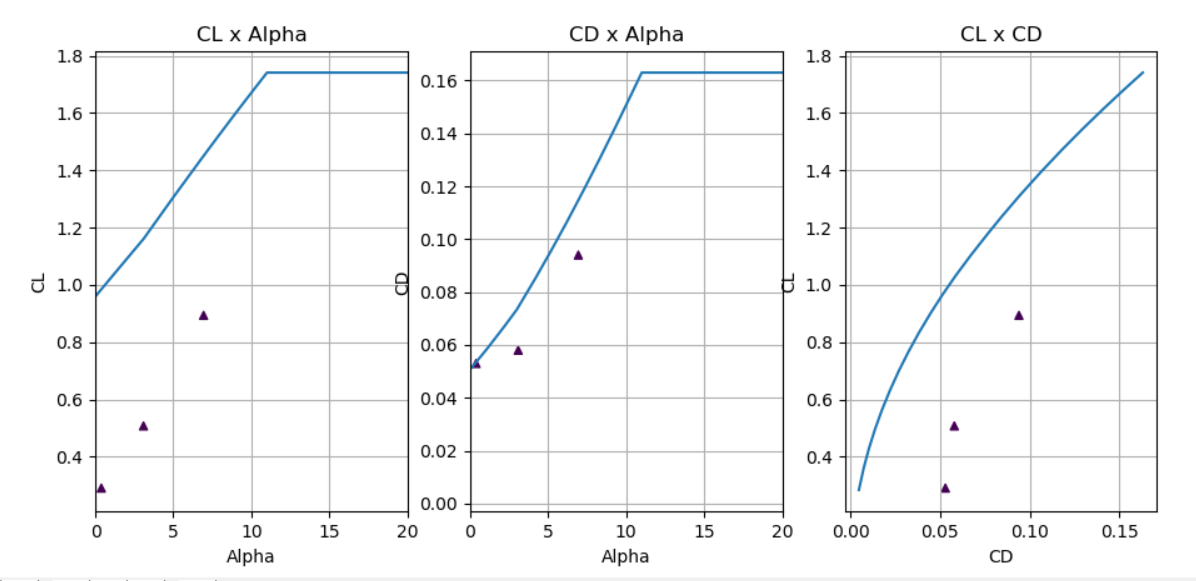
\includegraphics[width=.8\linewidth]{plots/cl_cd_polar_medicao.png}
    \caption{Curvas $C_x vs Alpha$, experimental e simulado. Fonte: O autor.}
    \label{fig:coefficients_alpha_plot}
\end{figure}

Os resultados do teste demonstram um alto desvio entre os valores de sustentação medidos experimentalmente e os simulados. Já os dados de arrasto se encontram próximos entre as duas fontes, porém com os dados experimentais sendo sempre menores que os simulados, ao contrario do que normalmente se espera, dado que os métodos de VLM costumam subestimar o arrasto.

Estes testes se mostraram inconclusivos, indicando apenas que existe pelo menos uma fonte de erro. Este erro pode estar vindo da própria bancada, por alguma falha construtiva ou de calibração, da execução do teste, por exemplo angulando-se o profundor de valor diferente do simulado, ou mesmo do protótipo, por falhas na construção. 

De fato tal aeronave indicou em testes de voo posteriores estar aparentemente com uma relação $C_L/C_D$ mais baixa do que o esperado, não conseguindo decolar com cargas maiores que 70\% daquela estimada em projeto, além de apresentar assimetria de sustentação entre os dois lados da asa, indicando diminuição da sustentação total gerada com relação aquela estimada em projeto.

Além disso os dados coletados aparentaram boa qualidade e relativa estabilidade, além de apresentarem comportamento coerente com o esperado. Erros na angulação do profundor, mesmo que altas, também não acarretariam em desvio tao grande dos valores de sustentação. Deste modo, parece provável um desvio do próprio protótipo em relação ao simulado, porém é importante que fique claro que tal hipótese não pode ser comprovada, dado que a bancada não foi validada contra valores conhecidos de literatura.


